\section{Suavidade (Tikhonov de ordem 1)}
\label{sec:smoothness}

Em certas situações é desejável que a distribuição dos parâmetros seja ``suave''.
Existem diversas interpretações para esta restrição, porém a mais comum é que
parâmetros espacialmente adjacentes devem ter valores mais próximos possível.
Em outras palavras, não devem haver variações abruptas entre parâmetros
espacialmente adjacentes, ou que a diferença entre estes parâmetros deve ser
mínima.
\\
\indent A função regularizadora utilizada para incorporar a informação de
suavidade tem a seguinte forma

\begin{equation}
\theta^{SV}(\vect{p}) = \vect{v}^T\vect{v} \thinspace ,
\end{equation}

\noindent em que $\vect{v}$ é um vetor com as diferêncas entre os parâmetros
espacialmente adjacentes. O vetor $\vect{v}$ é uma aproximação de diferenças
finitas para a derivada espacial dos parâmetros e pode ser escrito como

\begin{equation}
\vect{v} = \mat{R}\thinspace\vect{p} \thinspace ,
\label{eq:vetor_diferencas}
\end{equation}

\noindent em que $\mat{R}$ é uma matriz de diferenças finitas.

\begin{example}
Seja o problema inverso de estimar o relevo de uma bacia
sedimentar. Uma possível parametrização seria discretizar a bacia em 7 prismas
retangulares justapostos com larguras fixas. Os parâmetros a serem estimados
seriam então as 7 espessuras dos prismas (Figura \ref{fig:basin-smoothness}).
Impor suavidade ao relevo da bacia é equivalente a minimizar as diferenças
$p_1 - p_2$, $p_2 - p_3$, $p_3 - p_4$, $p_4 - p_5$, $p_5 - p_6$ e $p_6 - p_7$.
Neste caso, o vetor $\vect{v}$ das diferenças entre os parâmetros espacialmente
adjacentes é dado por

\begin{equation}
\vect{v} =
    \begin{bmatrix}
    p_1 - p_2 \\ p_2 - p_3 \\ p_3 - p_4 \\ p_4 - p_5 \\ p_5 - p_6 \\ p_6 - p_7
    \end{bmatrix}
    =
    \underbrace{
    \begin{bmatrix}
    1 & -1 & 0 & 0 & 0 & 0 & 0\\
    0 & 1 & -1 & 0 & 0 & 0 & 0\\    
    0 & 0 & 1 & -1 & 0 & 0 & 0\\    
    0 & 0 & 0 & 1 & -1 & 0 & 0\\    
    0 & 0 & 0 & 0 & 1 & -1 & 0\\    
    0 & 0 & 0 & 0 & 0 & 1 & -1\\    
    \end{bmatrix}}_{\mat{R}}    
    \underbrace{
    \begin{bmatrix}
    p_1 \\ p_2 \\ p_3 \\ p_4 \\ p_5 \\ p_6 \\ p_7
    \end{bmatrix}}_{\vect{p}}    
     \thinspace .
\end{equation}

\begin{figure}
    \centering
    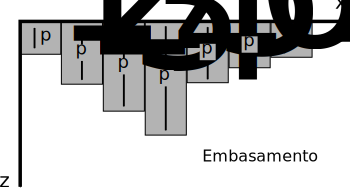
\includegraphics[scale=1]{figs/basin-smoothness}
    \caption{Exemplo de parametrização do relevo de uma bacia sedimentar.
    Neste caso, os 7 parâmetros utilizados são as espessuras de prismas
    retangulares justapostos. Impor suavidade ao relevo da bacia é equivalente
    a minimizar as diferenças $p_1 - p_2$, $p_2 - p_3$, $p_3 - p_4$, $p_4 - p_5$,
    $p_5 - p_6$ e $p_6 - p_7$.}
    \label{fig:basin-smoothness}
\end{figure}

\end{example}

\indent A {\it função regularizadora de suavidade} (também conhecida como
{\it Tikhonov de ordem um}) pode ser escrita como 

\begin{equation}
\theta^{SV}(\vect{p}) = \vect{p}^T \mat{R}^T \mat{R}\thinspace\vect{p} \thinspace .
\label{eq:suavidade}
\end{equation}

\noindent O vetor gradiente $\vect{\nabla}\theta^{SV}(\vect{p})$ e a matriz Hessiana
$\mat{\nabla}\theta^{SV}(\vect{p})$ (ver Apêndice \ref{chap:opmat}) desta função
são, respectivamente,

\begin{equation}
\vect{\nabla}\theta^{SV}(\vect{p}) = 2\mat{R}^T \mat{R}\thinspace\vect{p}
\end{equation}

\noindent e

\begin{equation}
\mat{\nabla}\theta^{SV}(\vect{p}) = 2\mat{R}^T \mat{R} \thinspace .
\end{equation}

\indent O gradiente da função regularizadora de norma mínima é uma
{\it combinação linear dos parâmetros}.
Para o caso em que a função $f_i(\vect{p})$ que relaciona
os dados preditos aos parâmetros também é {\it linear} (equação \ref{eq:comb_linear}),
a equação normal do {\it problema inverso linear regularizado},
para o caso da regularização de suavidade, é

\begin{equation}
\left(\mat{G}^T\mat{G} + \mu\mat{R}^T\mat{R}\right)\opt{p} =
    \mat{G}^T\left(\vect{d}^{\thinspace o} - \vect{b} \right) ,
\end{equation}

\noindent em que $\mu$ é o parâmetro de regularização, $\vect{d}^{\thinspace o}$
é o vetor de dados observados, $\mat{G}$ é a matriz de sensibilidade, $\vect{b}$
é um vetor de constantes (equação \ref{eq:f_igual_Gp}) e $\opt{p}$ é a solução
suave para o problema inverso linear.
\\
\indent Já para o caso em que $f_i(\vect{p})$ é {\it não-linear}, o problema
inverso torna-se também não-linear. Assim sendo, a equação normal do
{\it problema inverso não-linear regularizado}, para o caso da regularização de
suavidade, é

\begin{equation}
\left[\mat{G}(\vect{p}_0)^T\mat{G}(\vect{p}_0) +
      \mu\mat{R}^T\mat{R}\right]\Delta\vect{p} =
\mat{G}(\vect{p}_0)^T \left[\vect{d}^{\thinspace o} - \vect{f}(\vect{p}_0)\right] -
\mu\mat{R}^T\mat{R}\thinspace\vect{p}_0
    \thinspace .
\end{equation}

\noindent em que $\vect{f}(\vect{p}_0)$ é o vetor de dados preditos avaliado em
$\vect{p}_0$ e $\Delta\vect{p}$ é a correção a ser aplicada a $\vect{p}_0$.
